\documentclass{article}

% Package Information
\usepackage[margin=1in]{geometry}
\usepackage[hidelinks]{hyperref}
\usepackage{graphicx}
\usepackage{float}

% Title Information
\title{Overview of the Electrical Team}
\author{University of Calgary Solar Car Team\\
        Electrical Technical Documentation Team}
\date{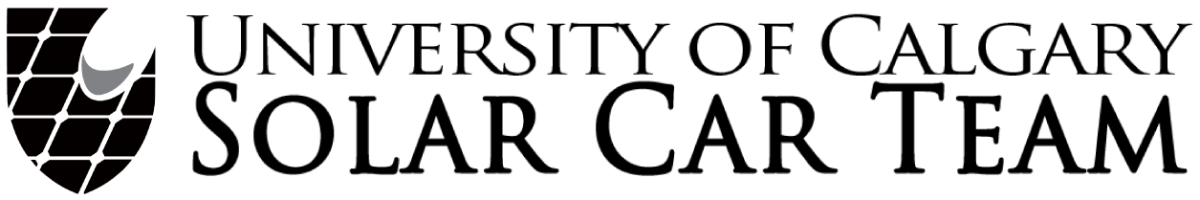
\includegraphics{images/logo.png}}

\begin{document}
    %\maketitle
    \begin{titlepage}
  
	    \newcommand{\HRule}{\rule{\linewidth}{0.5mm}} % Defines a new command for the horizontal lines, change thickness here
	    
	    \center % Center everything on the page
	     
	    %----------------------------------------------------------------------------------------
	    %	HEADING SECTIONS
	    %----------------------------------------------------------------------------------------
	    
	    \textsc{\LARGE University of Calgary Solar Car Team}\\[1.5cm] % Name of your university/college
	    \textsc{\Large Electrical Documentation}\\[0.5cm] % Major heading team name
	    
	    %----------------------------------------------------------------------------------------
	    %	TITLE SECTION
	    %----------------------------------------------------------------------------------------
	    
	    \HRule \\[0.4cm]
	      { \huge \bfseries Overview of the Electrical Team}\\[0.4cm] % Title of your document
	    \HRule \\[1.5cm]
	     
	    %----------------------------------------------------------------------------------------
	    %	AUTHOR SECTION
	    %----------------------------------------------------------------------------------------
	    
	    \Large \emph{Original Author:}\\
	    Andreas Smit\\[3cm] % Your name
	    
	    %----------------------------------------------------------------------------------------
	    %	DATE SECTION
	    %----------------------------------------------------------------------------------------
	    
	    {\large \today}\\[2cm] % Date, change the \today to a set date if you want to be precise
	    
	    %----------------------------------------------------------------------------------------
	    %	LOGO SECTION
	    %----------------------------------------------------------------------------------------
	    
	    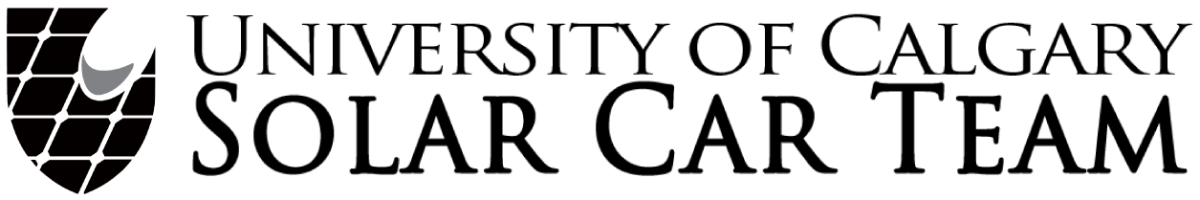
\includegraphics[width=\textwidth]{images/logo.png}\\[1cm] % Include a department/university logo - this will require the graphicx package
	     
	    %----------------------------------------------------------------------------------------
	    
	    \vfill % Fill the rest of the page with whitespace
  
	\end{titlepage}

    \section{Introduction}
    The electrical team deals with all of the electrical work for the
    University of Calgary Solar Car project. The electrical work can be
    broken down into roughly four basic areas of work; the four areas
    roughly are PCB design, the electrical systems, the battery system,
    and the solar arrays. 
    \section{PCB Design}
    The PCB work for the car is done by our PCB design team. All of our
    PCBs are designed in Altium PCB designer. A list of the PCBs 
    designed for the solar car is given below
    \begin{itemize}
        \item The AUX BMS
        \item The DC-DC Converter
        \item The CCS
        \item The Lights Board
        \item The Driver Control Board
        \item The CAN Spliter
        \item The Fan Board
        \item The Audio Board
        \item The Strobe Board
        \item The Relay Board
    \end{itemize}
    Some of the more complex boards will be discussed bellow
    \subsection{The Central Control System}
    The Central Control System or CCS is a board designed to control the
    CAN network of the car. The primary use of the CCS in the car is 
    sending data from the CAN network to the Raspberry Pis. A picture of
    the CCS hardware is given in figure \ref{fig:css}
    \begin{figure}[H]
        \centering
        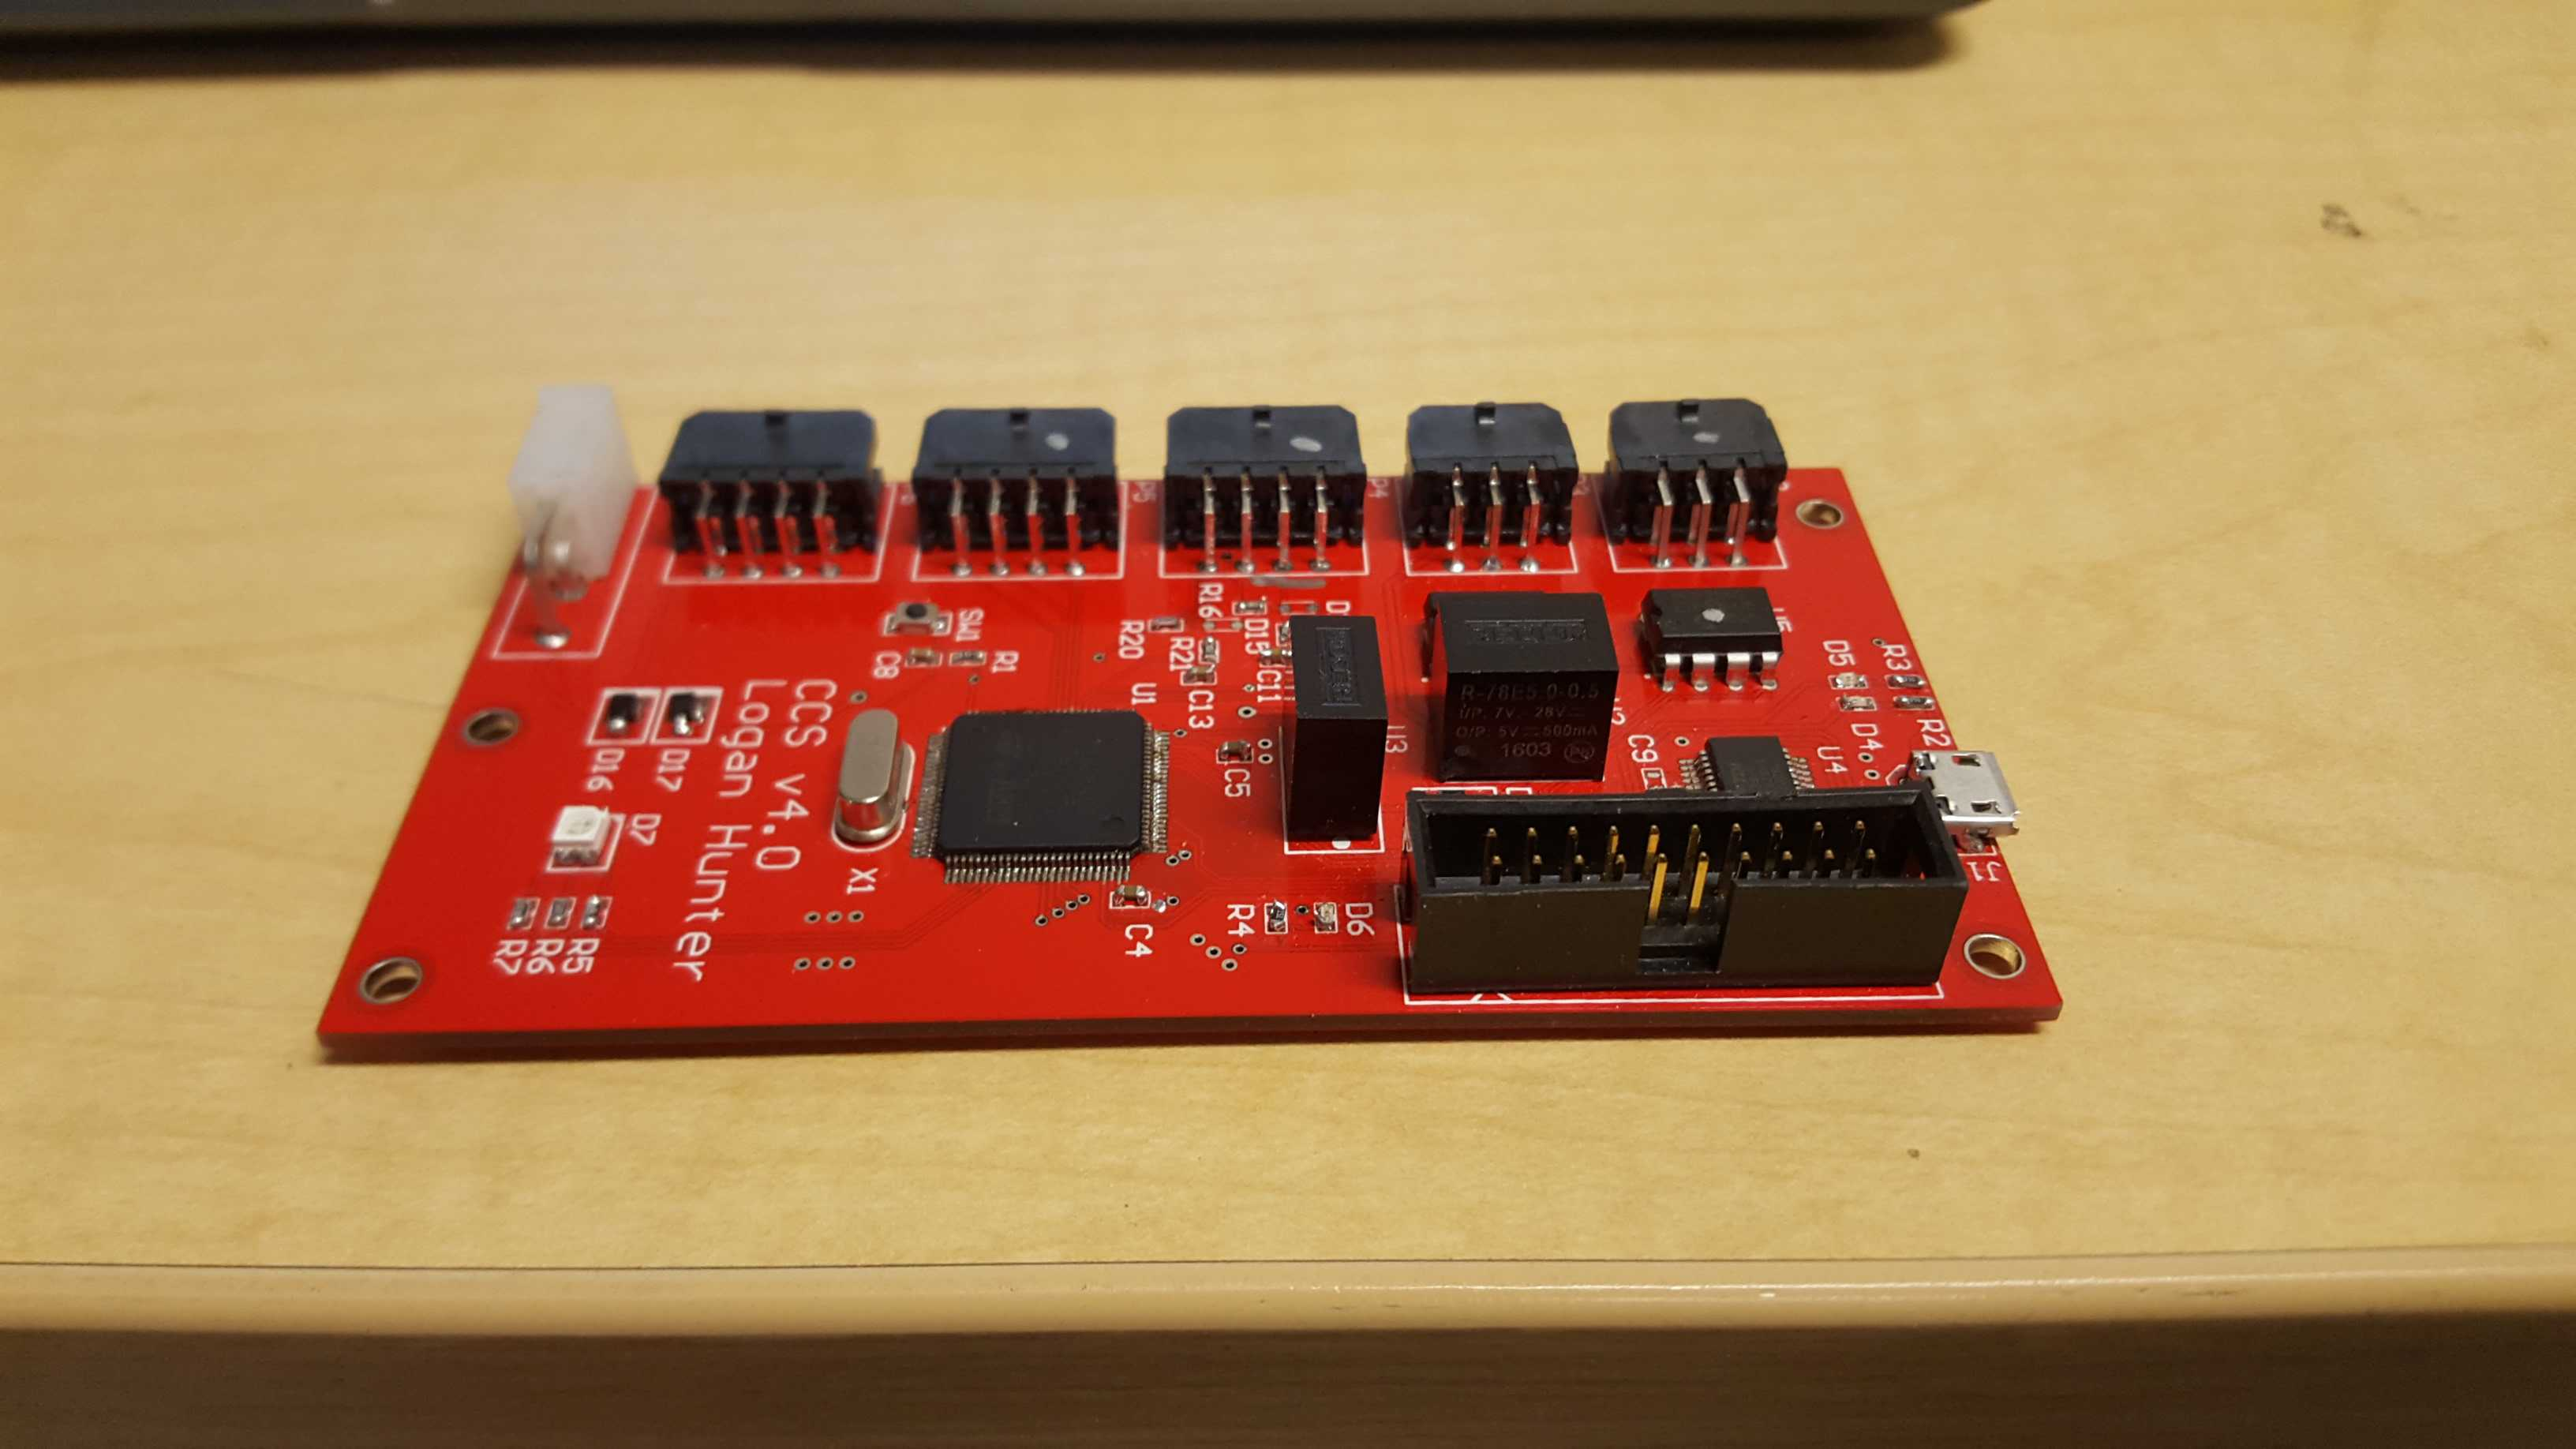
\includegraphics[width=0.5\textwidth]{images/ccs.jpg}
        \caption{The CCS board Hardware}
        \label{fig:css}
    \end{figure}
    \subsection{The Driver Control Board}
    The driver control board manages all driver inputs from the car and
    distributes the inputs over the CAN network. The inputs include but
    are not limited to acceleration and regen brake pedals, buttons for
    lights, drive control. A picture of the driver control hardware is
    given in figure \ref{fig:driver}
    \begin{figure}[H]
        \centering
        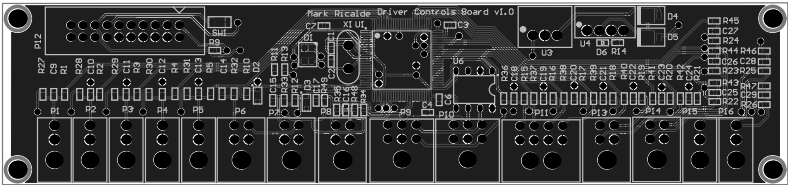
\includegraphics[width=0.5\textwidth]{images/driver.png}
        \caption{The Driver Control Hardware Schematic, as designed in
                 Altium}
        \label{fig:driver}
    \end{figure}
    \subsection{The Lights Board}
    The purpose of the lights board is to control all of the lights on
    the car, such as the headlights. The basic operation of the lights
    board the CAN network will tell the lights board which lights to
    turn on and then the board will send power to the necessary lights.
    Future upgrades that the team would want to make to the light board
    include integration of the emergency strobe board into the lights
    board and a sufficient power system to run the cars horn on. A
    picture of the lights board is given in figure \ref{fig:lights_HW}.
    \begin{figure}[H]
        \centering
        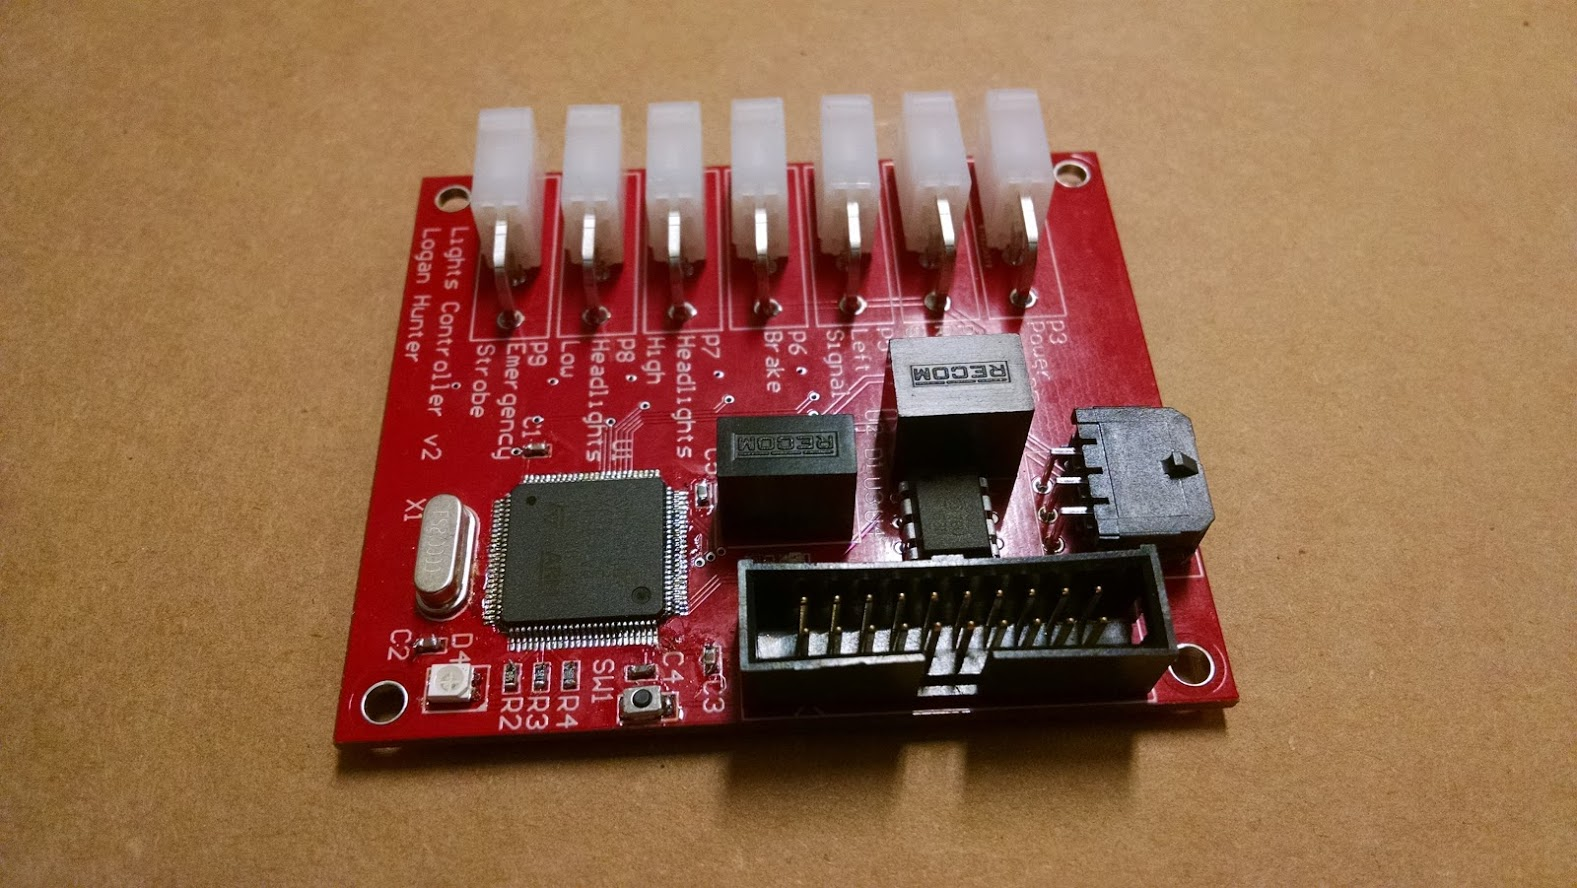
\includegraphics[width=0.5\textwidth]{images/light_board.jpeg}
        \caption{The Lights Board Hardware}
        \label{fig:lights_HW}
    \end{figure}
    \subsection{The Audio Board}
    The audio board will be used to add a media player into the solar
    car. It is designed to take aux input from a phone or other audio
    source and send it to two speakers which will be integrated into the
    car. The audio board is currently under active development. A
    picture of the audio board hardware is given in figure
    \ref{fig:audio}
    \begin{figure}[H]
        \centering
        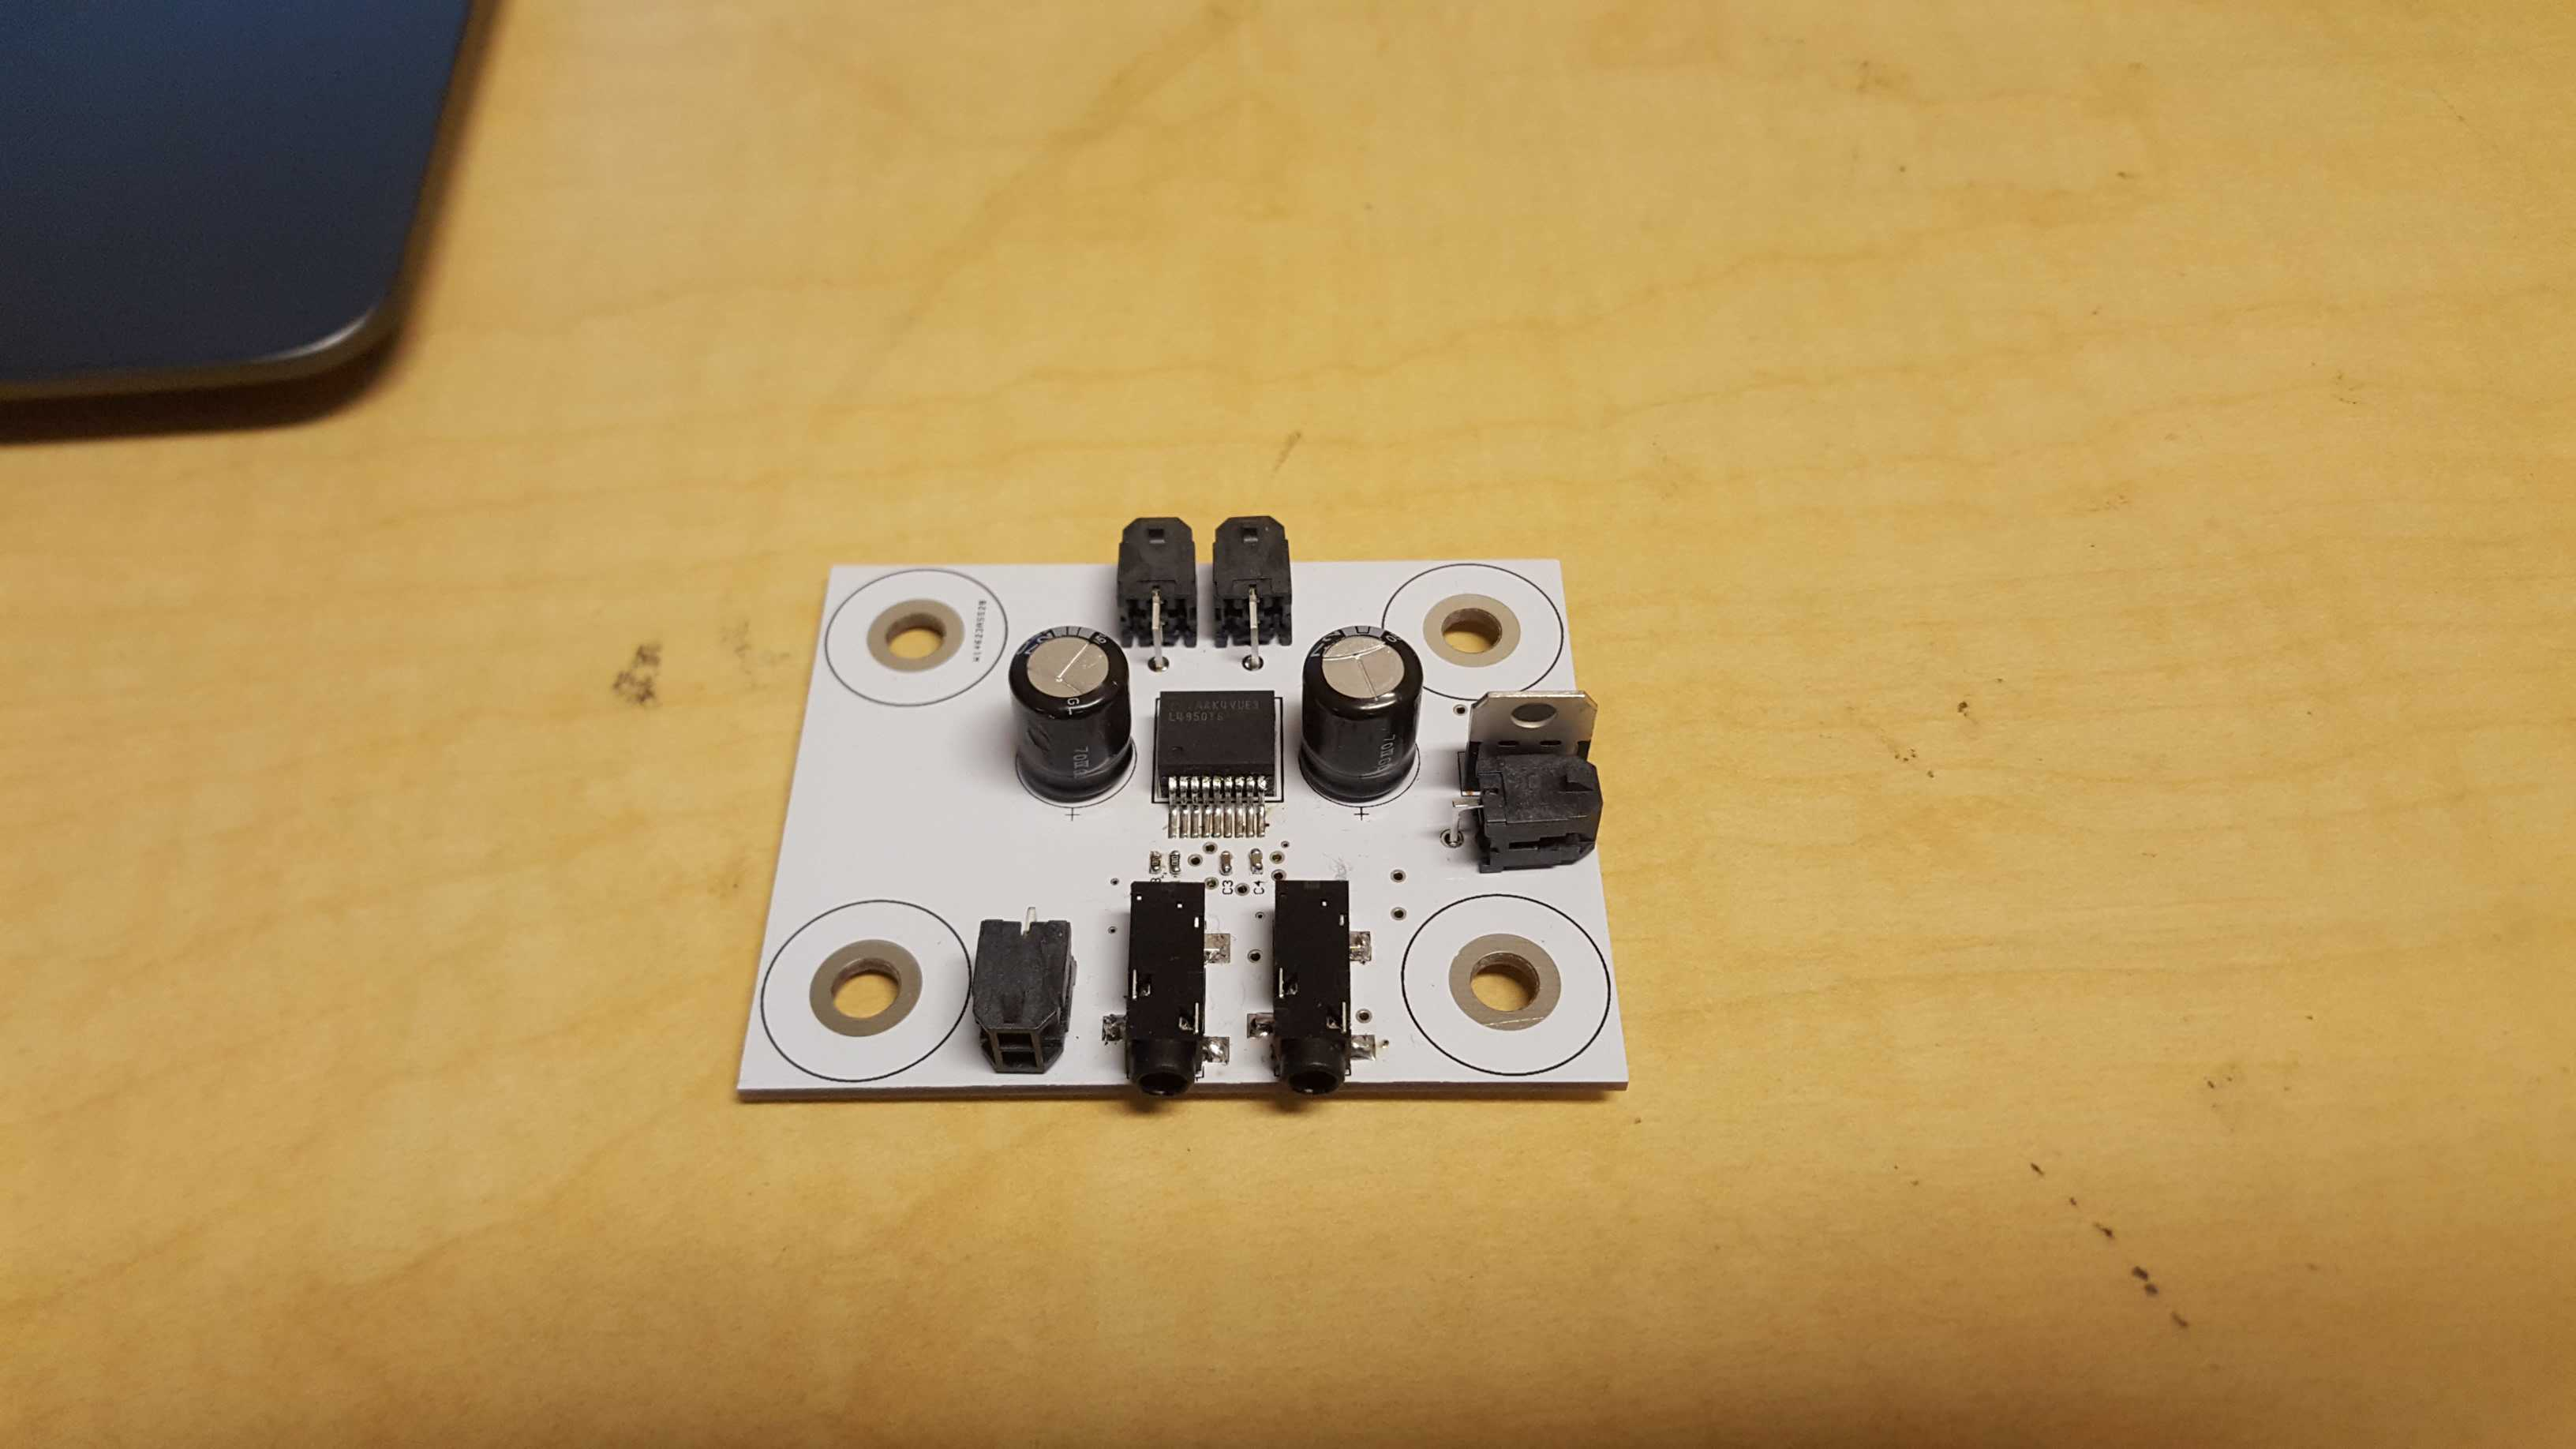
\includegraphics[width=0.5\textwidth]{images/audio_board.jpg}
        \caption{The Audio Board Hardware}
        \label{fig:audio}
    \end{figure}
    The AUX BMS and DC-DC converter will be talked about with the
    battery as they are directly inside the battery. The PCBs designed
    by the team for Elysia are estimated to have cost \$2000.

    % Systems Section
    \section{Electrical Systems}
    The electrical systems consist of the connection of all of the
    electrical components we make, such as the PCBs and battery, and the
    ones we purchase pre-made. All of our electrical devices in the car
    communicate over the CANbus network. One of the largest systems in
    the solar car is the high voltage system. A brief diagram of the
    cars electrical systems is shown in figure \ref{fig:systems}
    \begin{figure}[H]
        \centering
        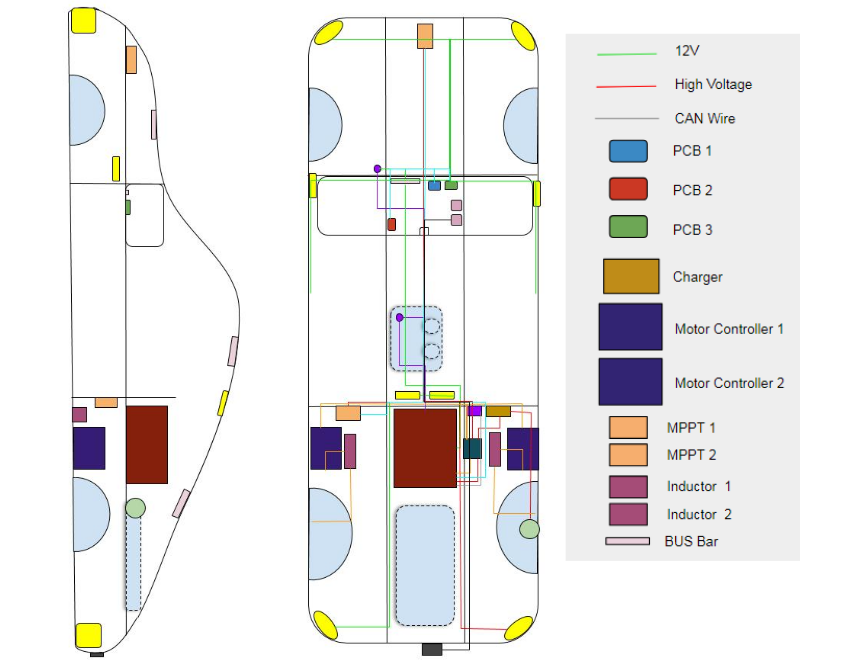
\includegraphics[width=\textwidth]{images/AllWiring.png}
        \caption{A rough schematic of the electrical systems in the car}
        \label{fig:systems}
    \end{figure}
    The high voltage system consists of our motors, the motor
    controllers, and the charge system. Multiple of the high voltage
    components are shown in figure \ref{fig:charge}
    \begin{figure}[H]
        \centering
        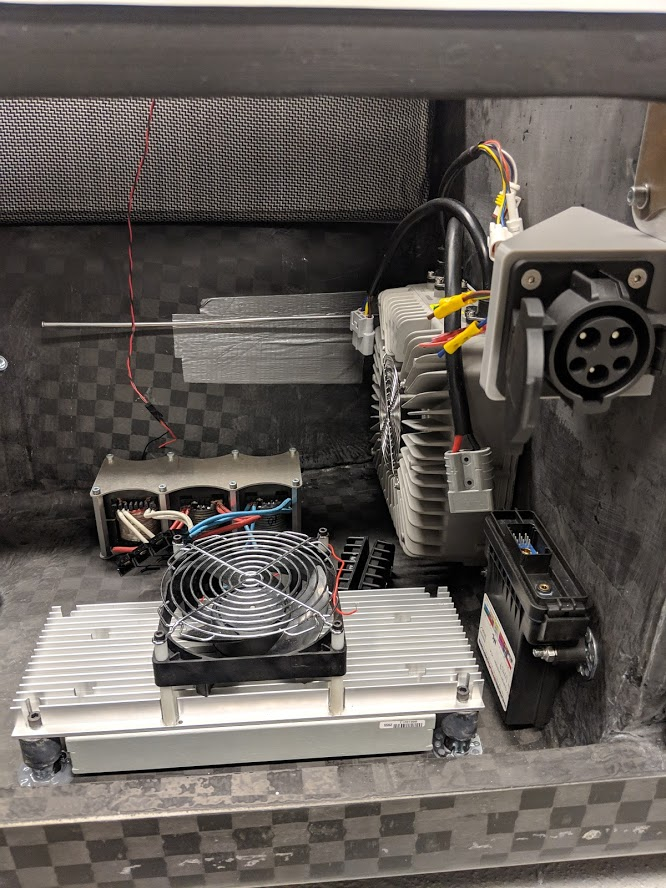
\includegraphics[width=0.5\textwidth]{images/car_internals.jpg}
        \caption{Some of the high voltage components of the car. Shown
            in the top right is the J1772 charging port, the bottom is
            one of the Tritium Wavesculpter 22 Motor Controllers, behind
            the motor controller is the motor inductors, and on the
        right is the charger and charge controller.}
        \label{fig:charge}
    \end{figure}
    The motor controllers used in the car are Tritium Wavesculpter 22s.
    There is two motor controllers, one for each of the two motors. The
    internals of the motor controller are shown in figure
    \ref{fig:mc}. Each of the motor controllers costs about \$4 500
    \footnote{All prices are given in USD unless otherwise stated}.
    With our next generation vehicle we are planning to replace the
    current motor controllers.
    \begin{figure}[H]
        \centering
        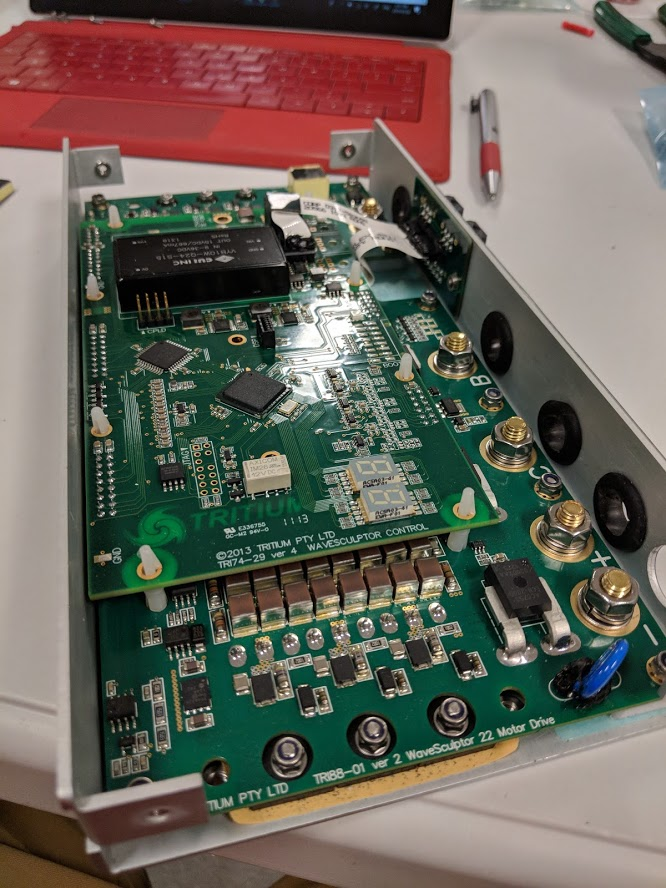
\includegraphics[width=0.5\textwidth]{images/mc_inside.jpg}
        \caption{The internals of one of our Tritium Wavesculpter 22
            Motor Controllers}
        \label{fig:mc}
    \end{figure}
    The motors used in the car are Marand Arial Flux Surface Mount
    Motors. The motors are $98.7\%$ efficient. They are 3 phase
    brushless DC motors that sit in the wheel hub. The motors can drive
    the car at up to $95\ km/h$. A picture of our motors are shown in
    figure \ref{fig:motor}.
    \begin{figure}[H]
        \centering
        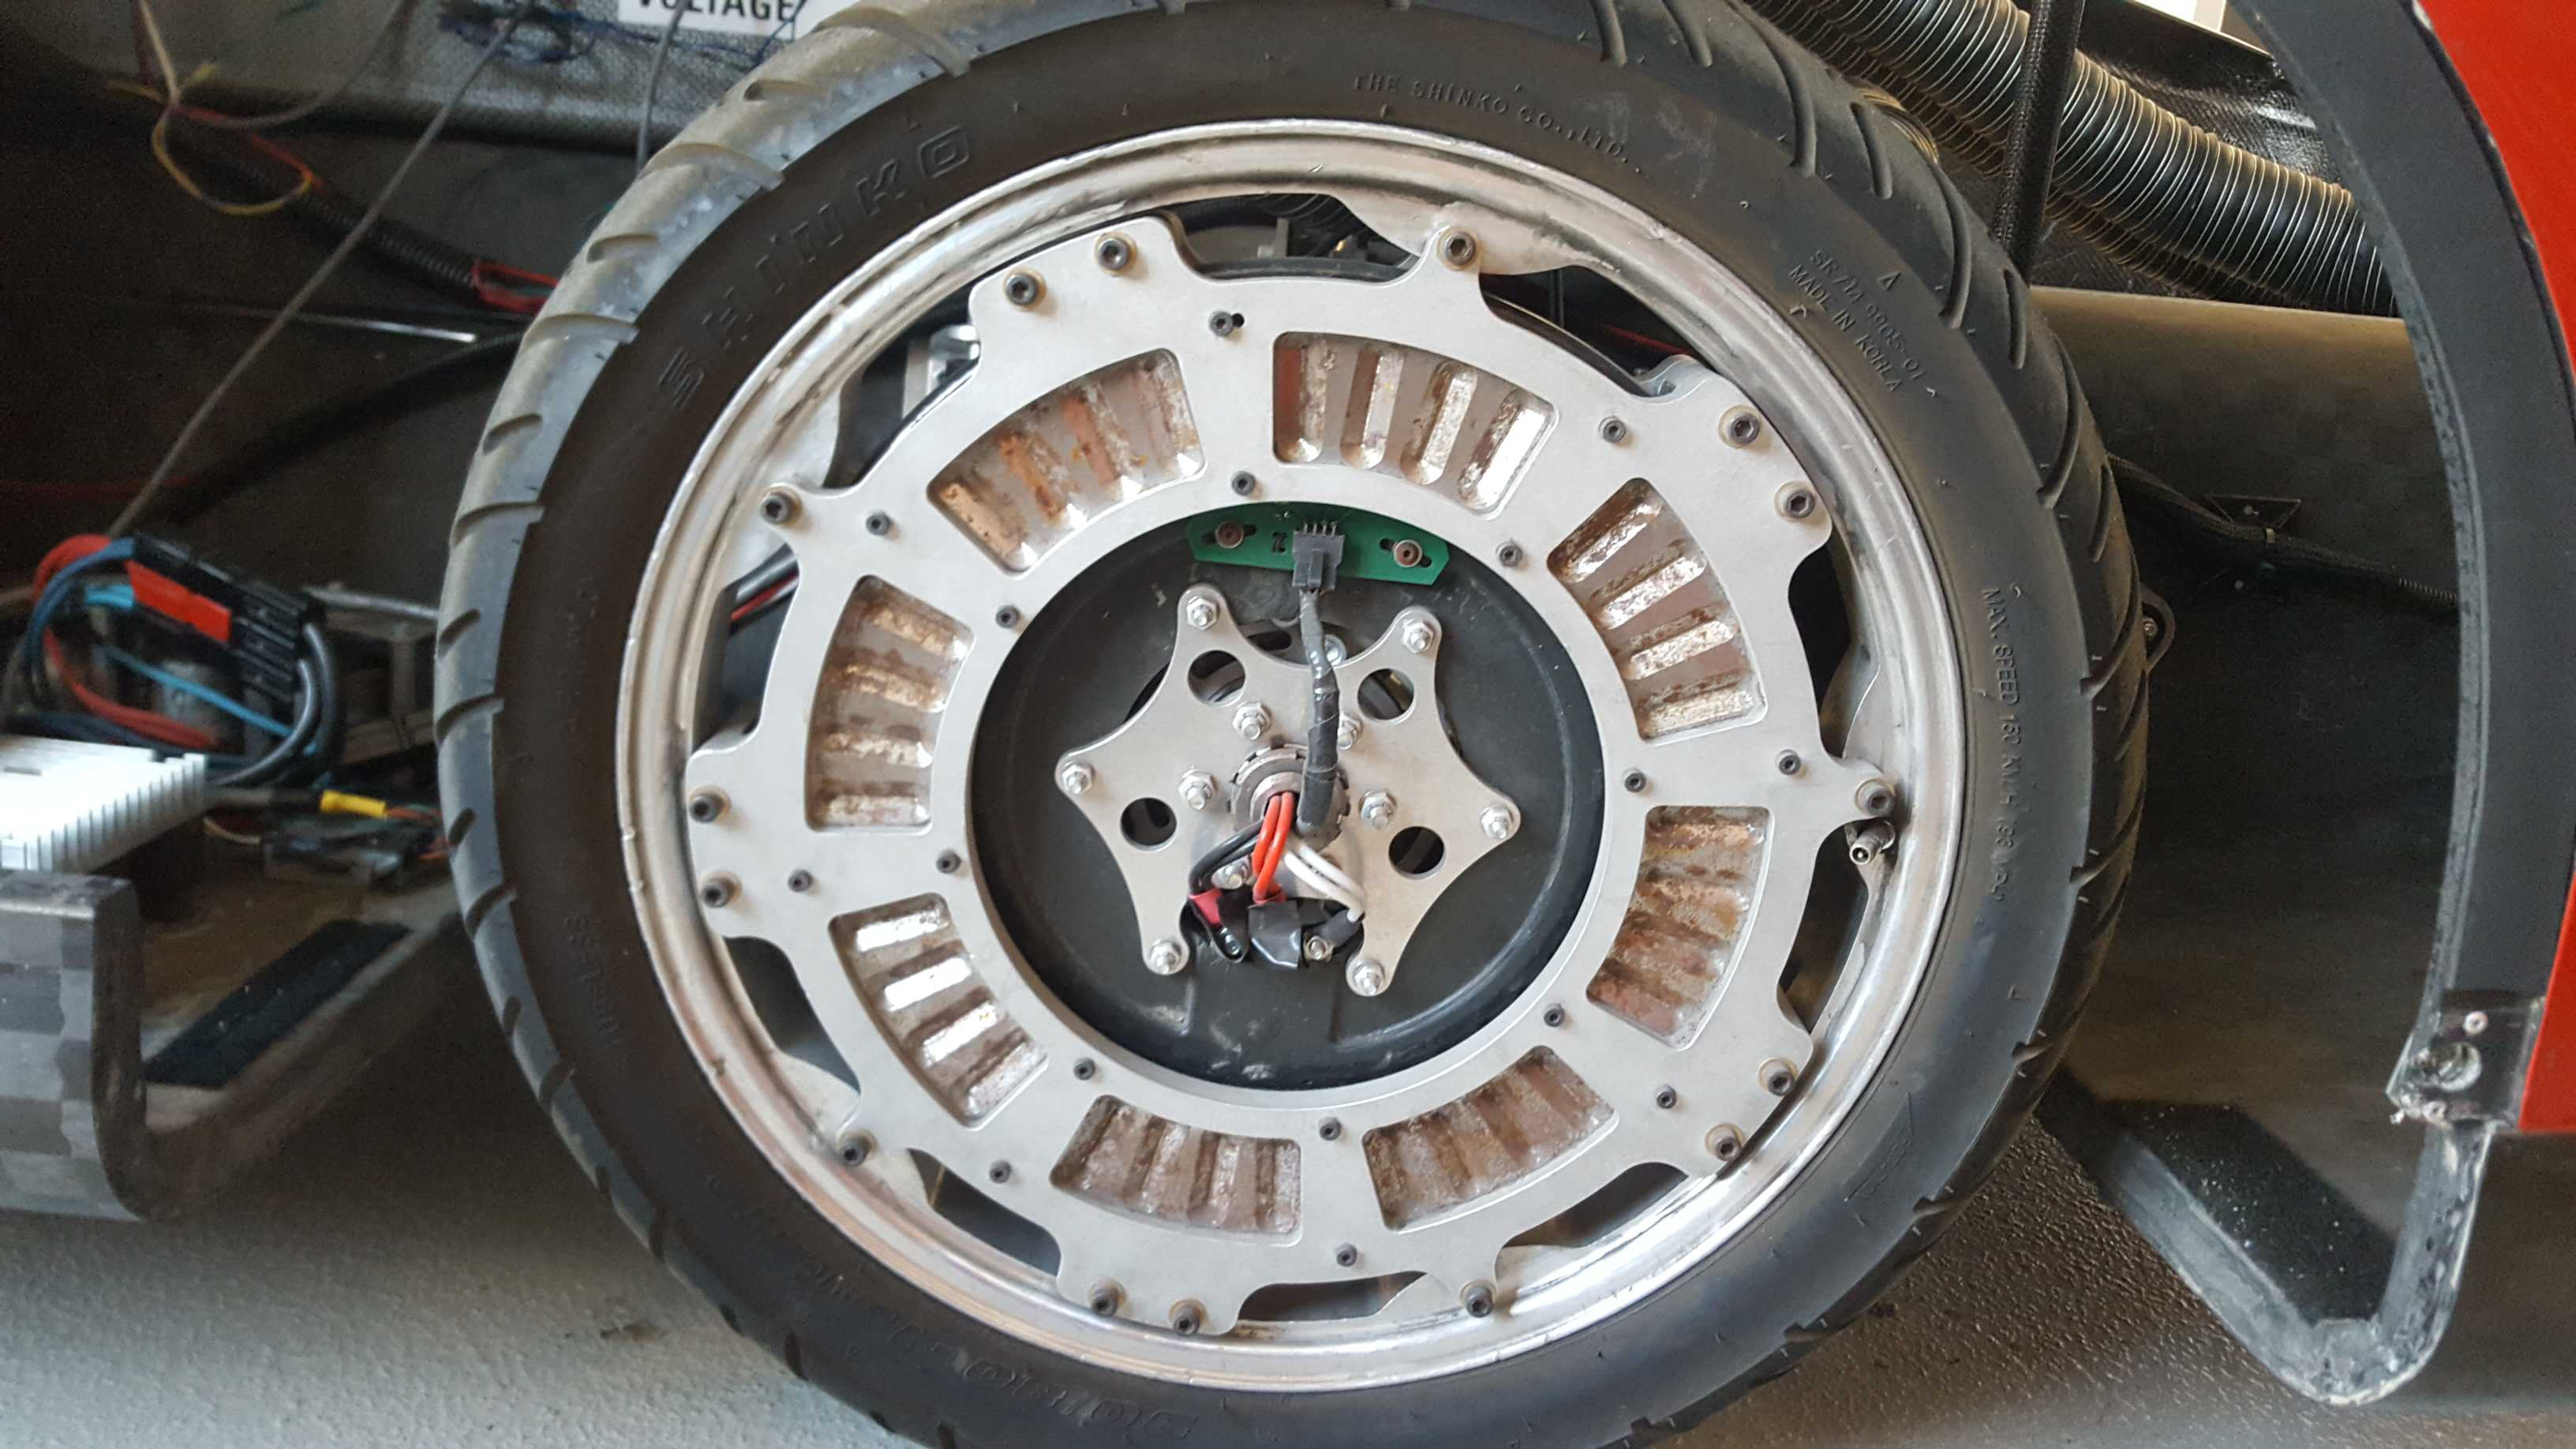
\includegraphics[width=0.5\textwidth]{images/motor.jpg}
        \caption{The motors built into the back wheel}
        \label{fig:motor}
    \end{figure}
    \noindent In the next generation car we are looking to replace our
    motors with an estimated cost of \$40 000 per motor.\\\\
    \par Another of the major systems in the car is the lights system.
    The lights are all turned on or off through the lights control board.
    The lights on the car are head lights, left signals, right signals,
    rear lights, break lights, and the emergency strobe light. There is
    plans to add interior lights to the car for at demo events. A
    picture of the car with the lights on is shown in figure
    \ref{fig:lights}
    \begin{figure}[H]
        \centering
        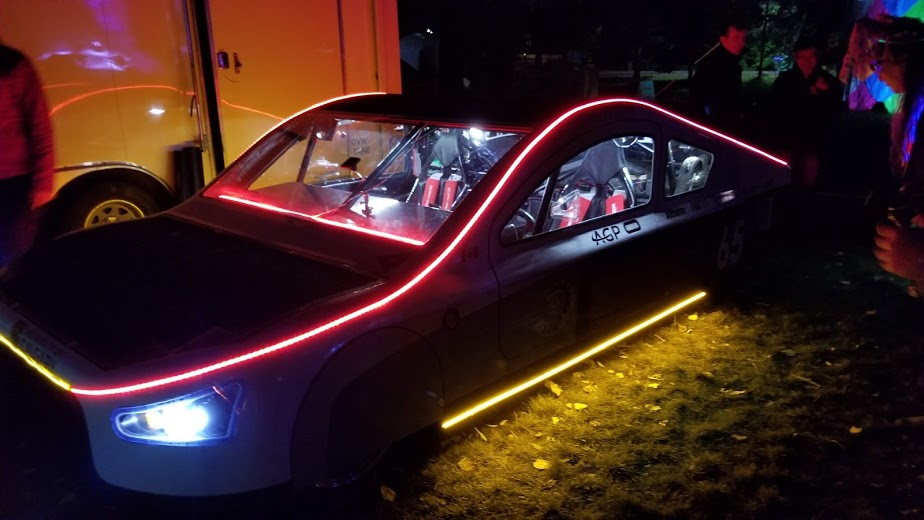
\includegraphics[width=0.75\textwidth]{images/lights.jpg}
        \caption{A picture of the solar car with all of its lights on
        from Beakerhead 2019}
        \label{fig:lights}
    \end{figure}

    % Battery
    \section{Battery Systems}
    The battery provides the electrical power for the car. The battery
    consists of a $10 000\ mAh$ nickle metal hydride auxiliary battery,
    and 1440 18650s lithium ion battery cells. Each lithium cell costs
    around \$4 leading to a total cost of around \$5760. The total
    capacity of the batter is $18\ kWh$ which is around the total daily
    energy usage of a typical Albertan household per day. The battery
    can output $126\ V$ at up to $230\ A$. All 1440 lithium cells are
    shown in figure \ref{fig:bat_cells}.
    \begin{figure}
        \centering
        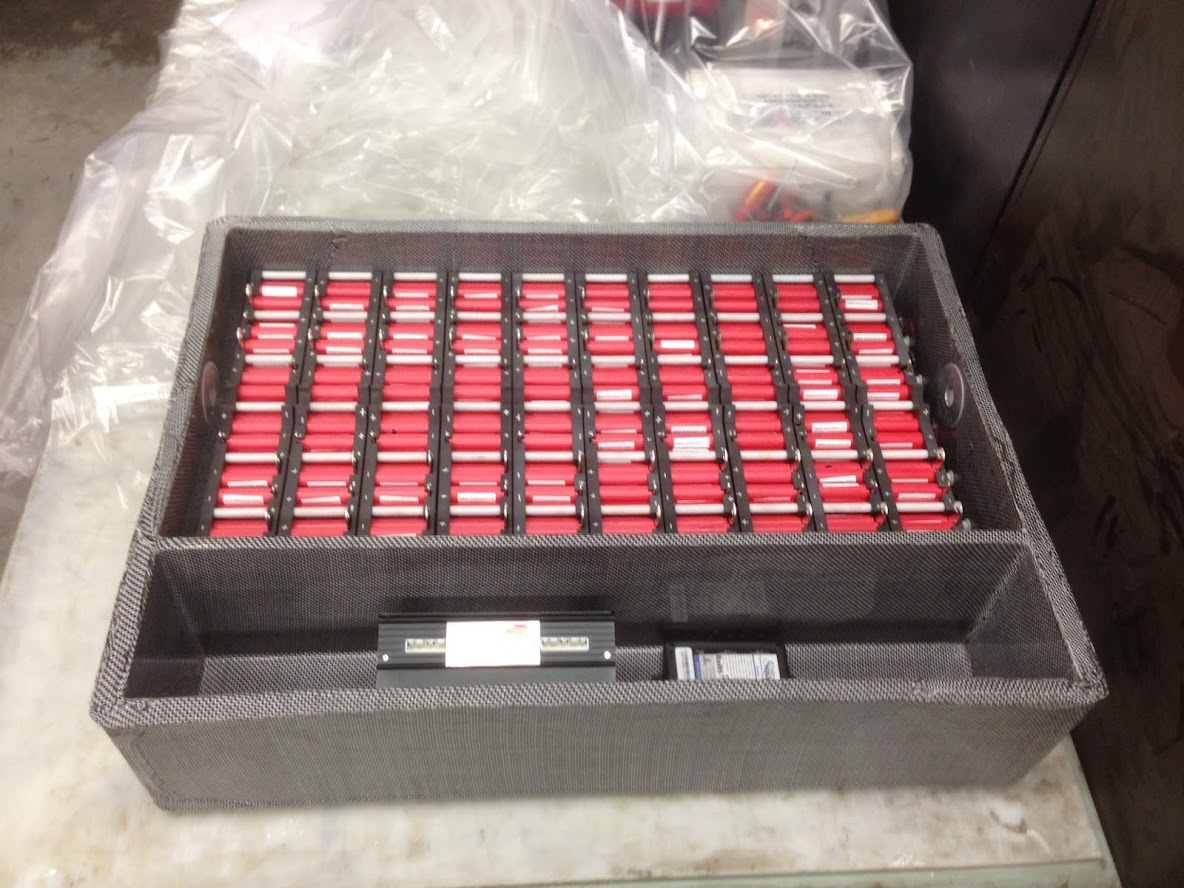
\includegraphics[width=0.5\textwidth]{images/cells.jpg}
        \caption{The 18650 battery cells in the battery casing}
        \label{fig:bat_cells}
    \end{figure}
    On top of the batteries in the battery box there is also safety
    equipment to ensure the safe operation of the battery. The major
    components in the battery protection system are the Orion battery
    management system (BMS), the Aux Battery management system PCB
    (AUX BMS), the DC to DC converter PCB and the aux battery itself.
    The internal electrics of the battery can be seen in figure
    \ref{fig:bat-in}.
    \begin{figure}[H]
        \centering
        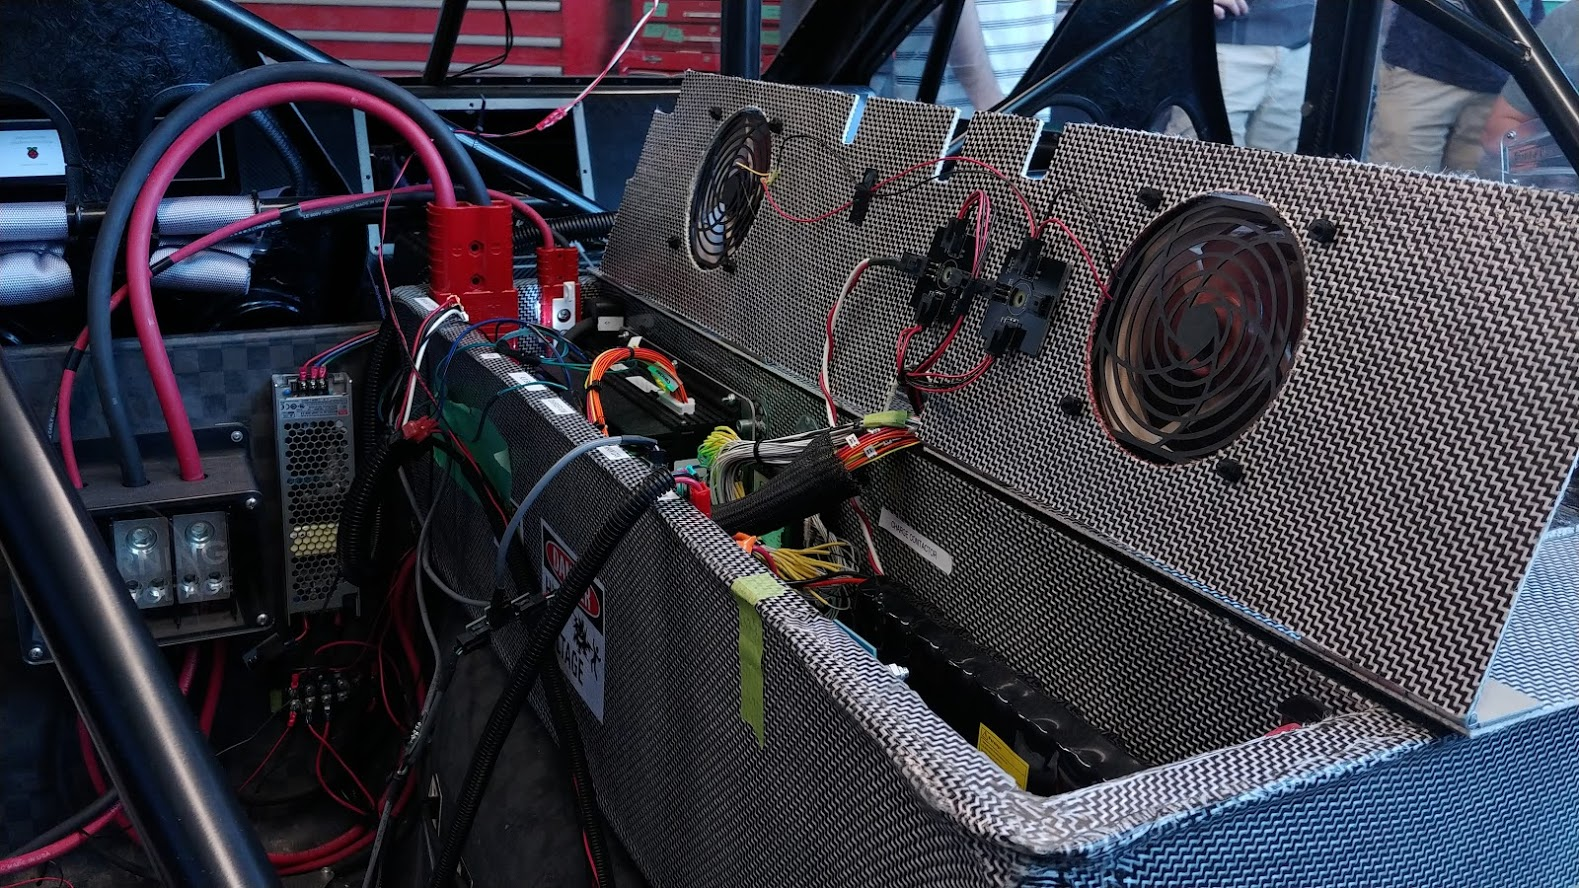
\includegraphics[width=0.5\textwidth]{images/batt-elec.jpg}
        \caption{The insides of the battery}
        \label{fig:bat-in}
    \end{figure}
    The Orion Battery management systems main job is to monitor the
    temperature, voltage, and current output of the battery. Should any
    of the expected values ever become unsafe it will send a message to
    the AUX BMS board. The Orion BMS costs around \$3 000.\\
    \par The AUX BMS has three major jobs. The first of its jobs is
    monitoring the AUX battery output. The second and more important is
    monitoring the output of the main BMS. In the event that the BMS
    detects a battery system fault the AUX BMS will open the 3
    contactors connecting the battery to the rest of the car. This
    isolates the battery from the rest of the car, preventing damage or
    electric discharge through the body of the car. The final job of the
    AUX BMS is to check if the main battery is safe to start when turn
    the car on. During this time it is powered from the aux battery. The
    aux bms was designed by the team in altium as shown in figure
    \ref{fig:aux-bms-alt}
    \begin{figure}[H]
        \centering
        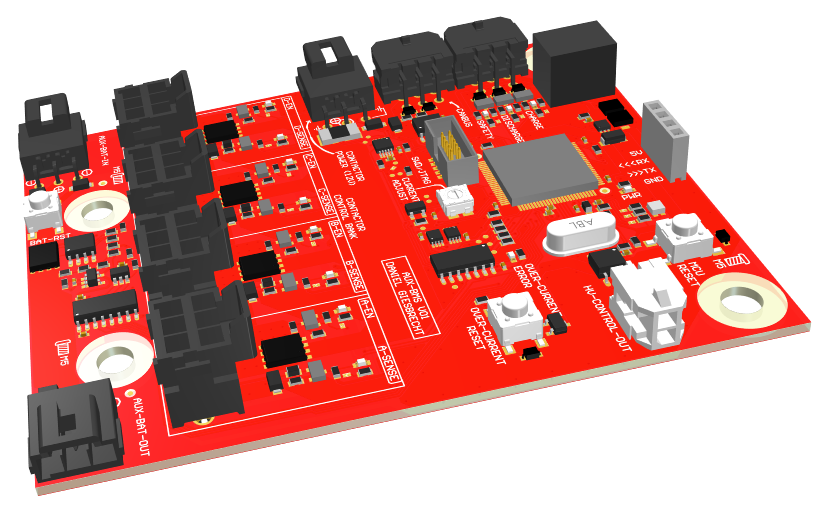
\includegraphics[width=0.5\textwidth]{images/aux_bms_alt.png}
        \caption{The aux BMS being displayed in Altium Designer}
        \label{fig:aux-bms-alt}
    \end{figure}
    \noindent After the design in altium our final PCB is shown in
    figure \ref{fig:aux-bms}
    \begin{figure}[H]
        \centering
        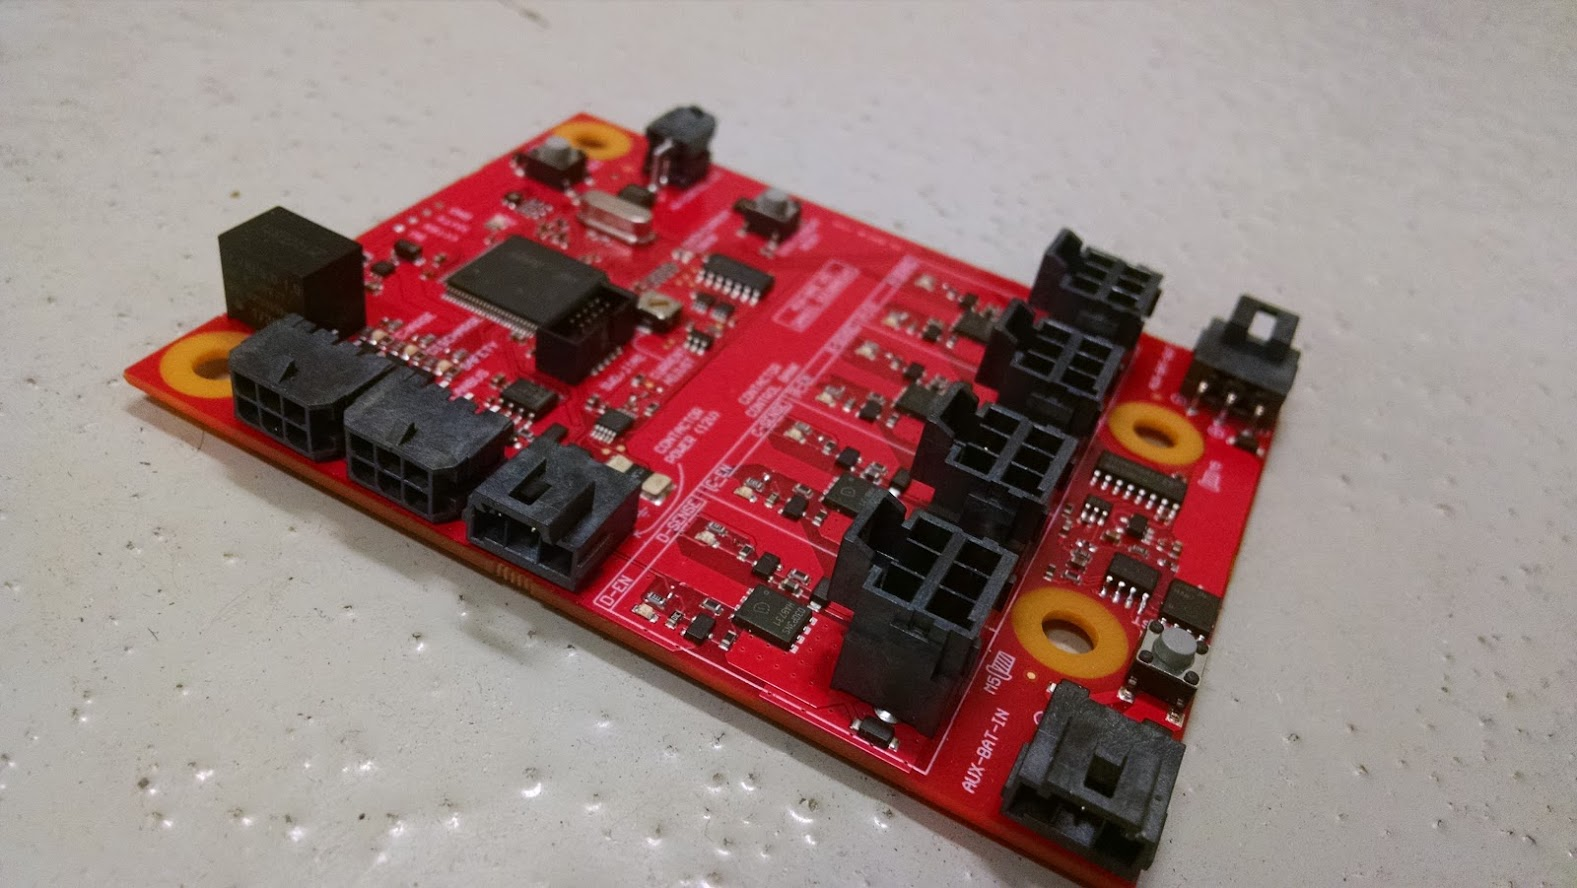
\includegraphics[width=0.5\textwidth]{images/aux_bms.jpeg}
        \caption{Aux BMS hardware}
        \label{fig:aux-bms}
    \end{figure}
    \par The DC to DC boards primary job is to convert the $120\ V$ DC
    from the battery pack to $12\ V$ DC for the PCBs and CAN bus in the
    car to be powered from. It also converts the approximate $12\ V$
    output of the Aux Battery into exactly $12\ V$ to power the aux BMS
    in the startup of the car and during an emergency shutdown. The
    DC-DC board was designed by the solar car team in Altium Designer.
    The board is shown in figure \ref{fig:DCDC}
    \begin{figure}[H]
        \centering
        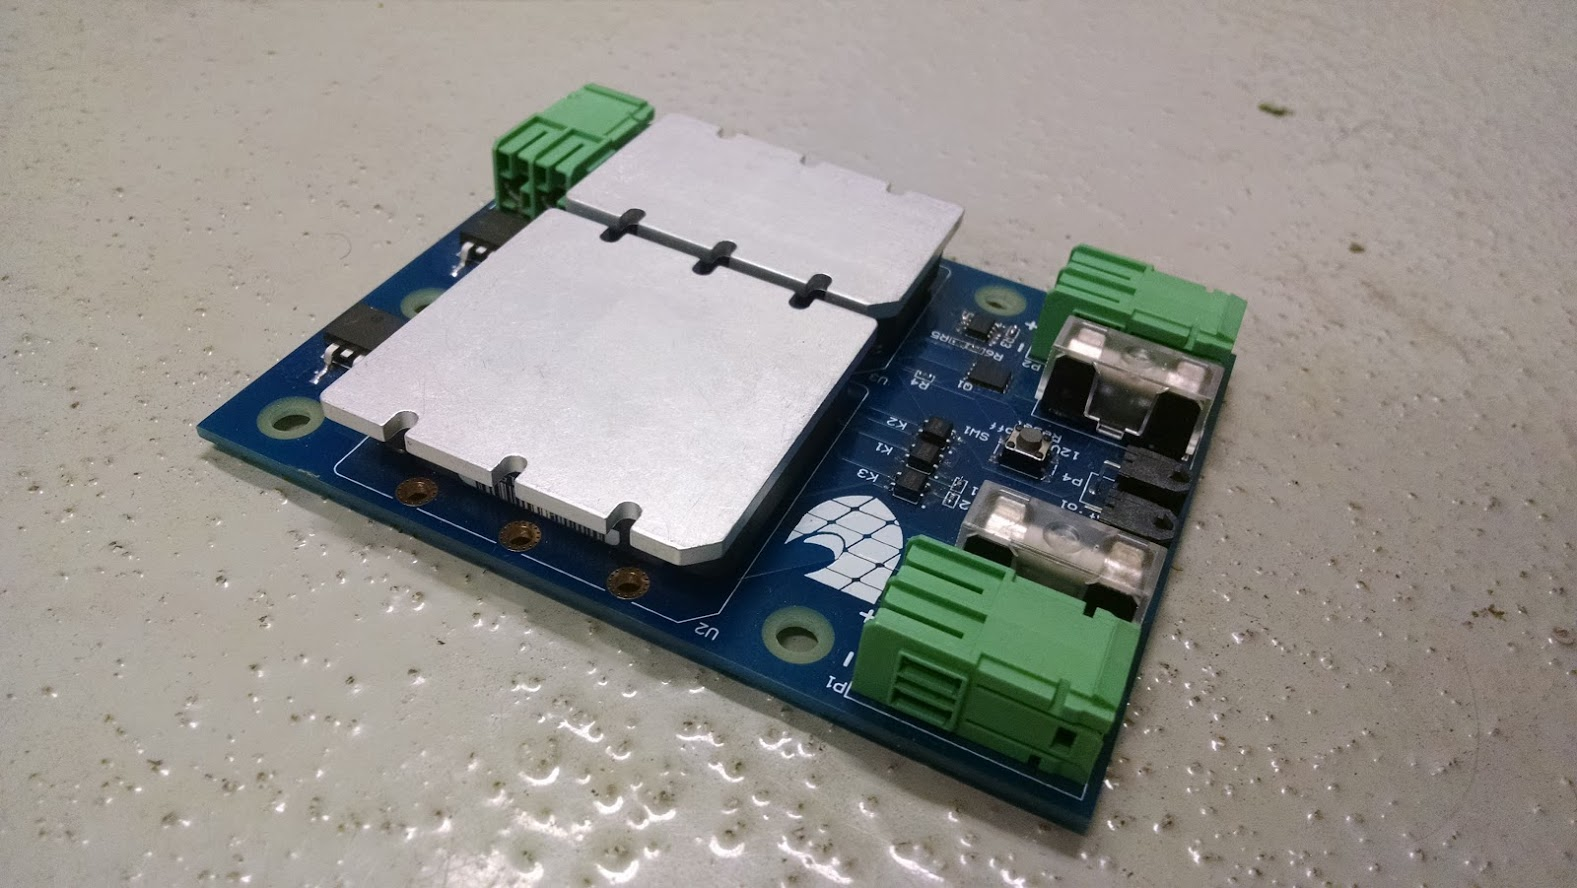
\includegraphics[width=0.5\textwidth]{images/dc-dc_board.jpeg}
        \caption{The DC to DC board}
        \label{fig:DCDC}
    \end{figure}
    \par As all the electronics in the battery box can get hot, there is
    8 cooling fans to help cool the battery. 6 of the fans pull air out
    of the main compartment where all 1440 lithium ion cells are; As per
    the solar car race regulations, we can not push air into the area
    with the lithium cells with fans for fear of a fire. Instead air is
    pushed in to the battery compartment through side vents on the car
    as we drive in race. 2 additional fans are used cool the safety
    electronics with one pushing air in and one pulling air out. The
    fans can be seen in figure \ref{fig:fans}
    \begin{figure}[H]
        \centering
        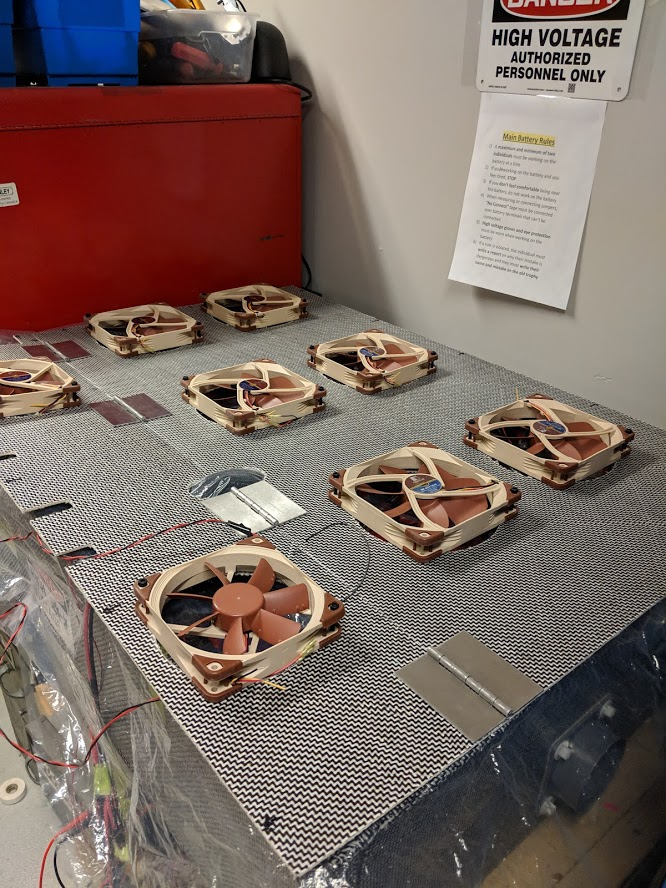
\includegraphics[width=0.5\textwidth]{images/fans.jpg}
        \caption{The 8 battery cooling fans}
        \label{fig:fans}
    \end{figure}
    \section{Solar Arrays}
    The solar panels are what convert our car from an electric car, to a
    solar car. The car has approximately $5\ m^2$ of solar panels
    covering its upper surfaces. All the solar panels on our car are
    encapsulated to increase the efficiency of the panels; Encapsulation
    is the process by which our panels are coated with tiny prisms to
    refract the light more perpendicularly into the panels. The power
    transfer from the arrays is controlled through two Max Power Point
    Trackers or MPPTs. The Schulich Elysia uses two Dilithium Photon 3
    MPPTs, valued at \$2200 a piece. The MPPTs tracks the power output
    of the array, and dictates the voltage and current to maximize the
    power output as shown in figure \ref{fig:mppt-graph}
    \begin{figure}[H]
        \centering
        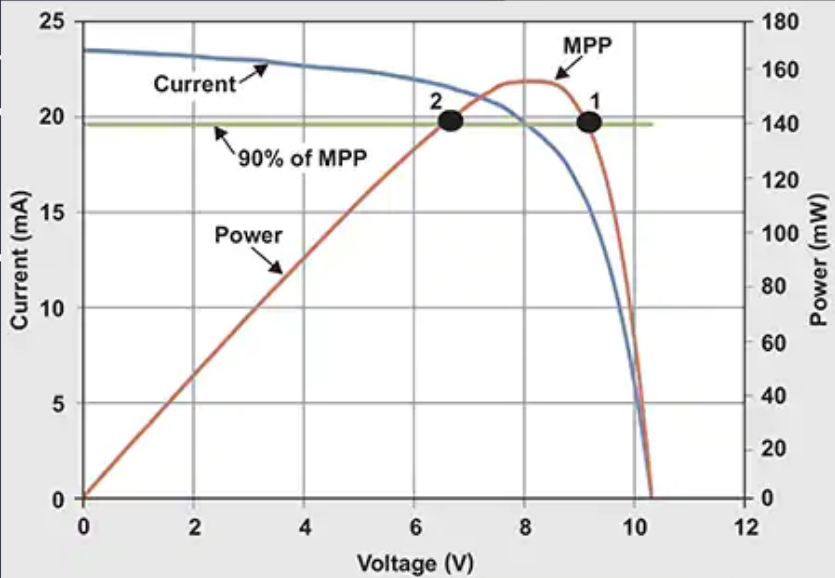
\includegraphics[width=0.5\textwidth]{images/MPPT_Diagram.png}
        \caption{The graph of Power vs Voltage for the MPPTs}
        \label{fig:mppt-graph}
    \end{figure}
    A picture of one the Dilithium Photon 3 MPPT is shown in figure
    \ref{fig:mppt}
    \begin{figure}[H]
        \centering
        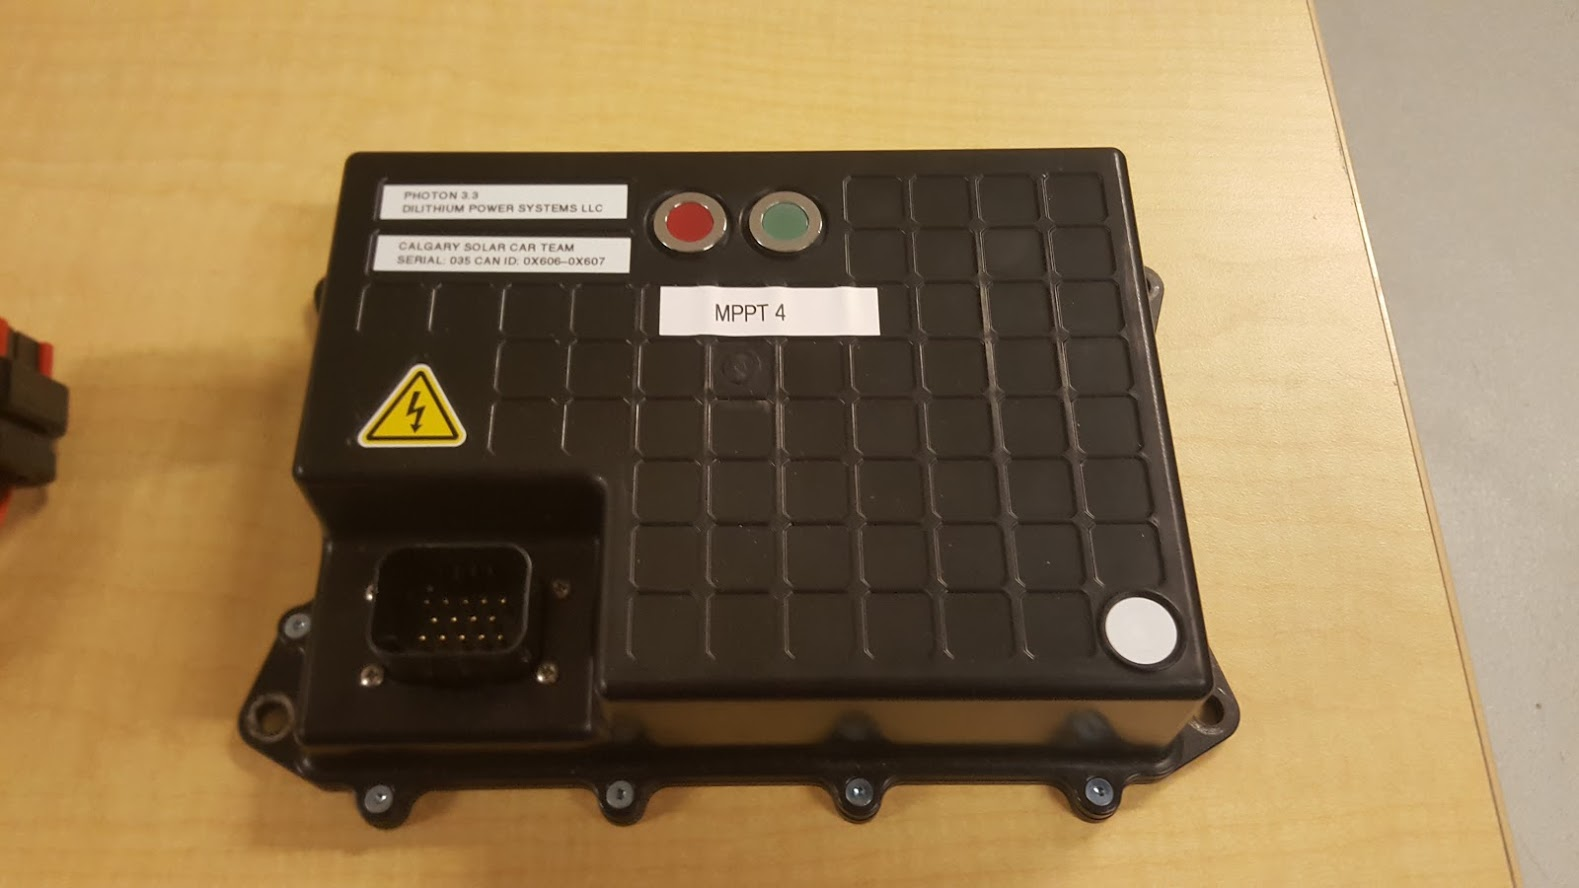
\includegraphics[width=0.5\textwidth]{images/mppt.jpg}
        \caption{One of the MPPTs used in Elysia}
        \label{fig:mppt}
    \end{figure}
    The solar arrays on the car cost around \$100 000. Figure
    \ref{fig:arr_schem} shows the schematic of how our arrays are wired
    into the car.
    \begin{figure}[H]
        \centering
        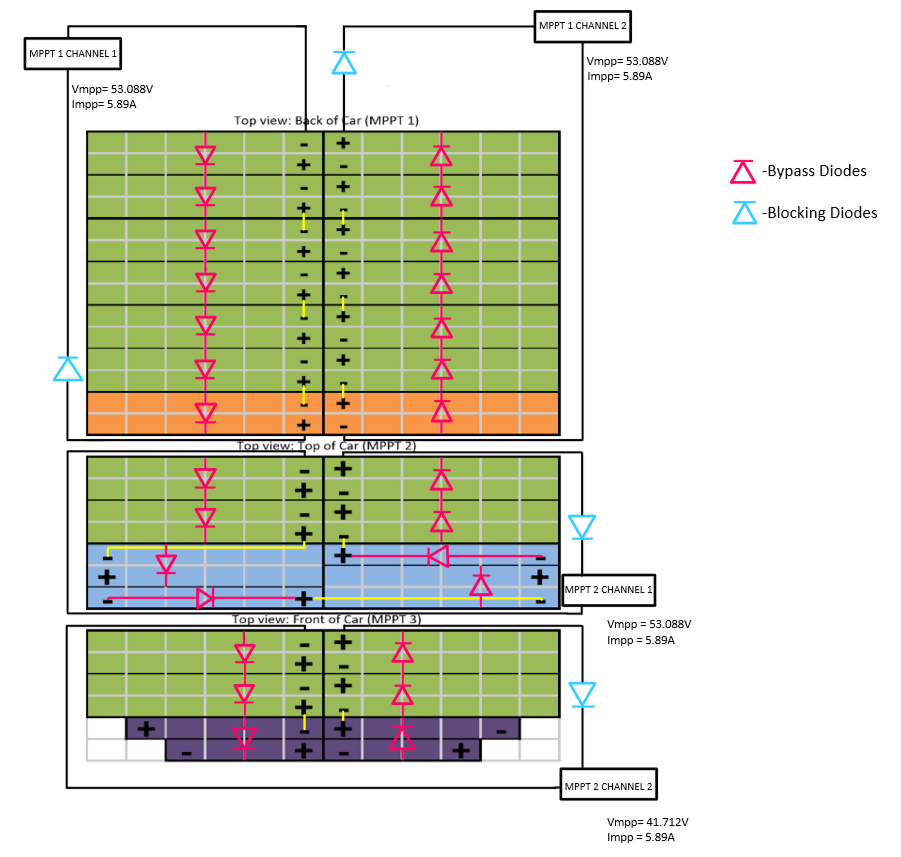
\includegraphics[width=0.5\textwidth]{images/array_schem.png}
        \caption{The schematic of the solar arrays in the car}
        \label{fig:arr_schem}
    \end{figure}
    \noindent The array on the car is shown in figure \ref{fig:array}
    \begin{figure}[H]
        \centering
        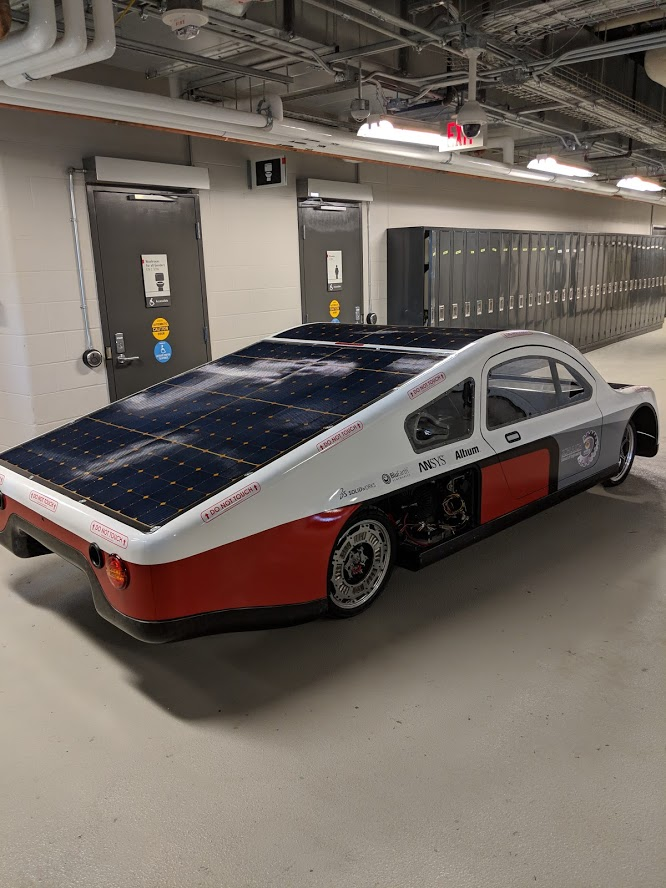
\includegraphics[width=\textwidth]{images/array.jpg}
        \caption{The Arrays on the back of Schulich Elysia}
        \label{fig:array}
    \end{figure}
\end{document}
